% Please do not change the document class
\documentclass{scrartcl}

% Please do not change these packages
\usepackage[hidelinks]{hyperref}
\usepackage[none]{hyphenat}
\usepackage{setspace}
\usepackage{graphicx}
\doublespace

% You may add additional packages here
\usepackage{amsmath}

% Please include a clear, concise, and descriptive title
\title{Usability Analysis}

% Please do not change the subtitle
\subtitle{COMP140 - Usability Analysis}

% Please put your student number in the author field
\author{1507290}

\begin{document}

\maketitle

\abstract{}
\section{Introduction}
This report will analyse usability issues raised in an evaluation of a controller for \textit{Hotrod the Beetle} that relate to the controller's use of LEDs and its interaction with the game.

\section{The Controller}
\begin{figure}[h]
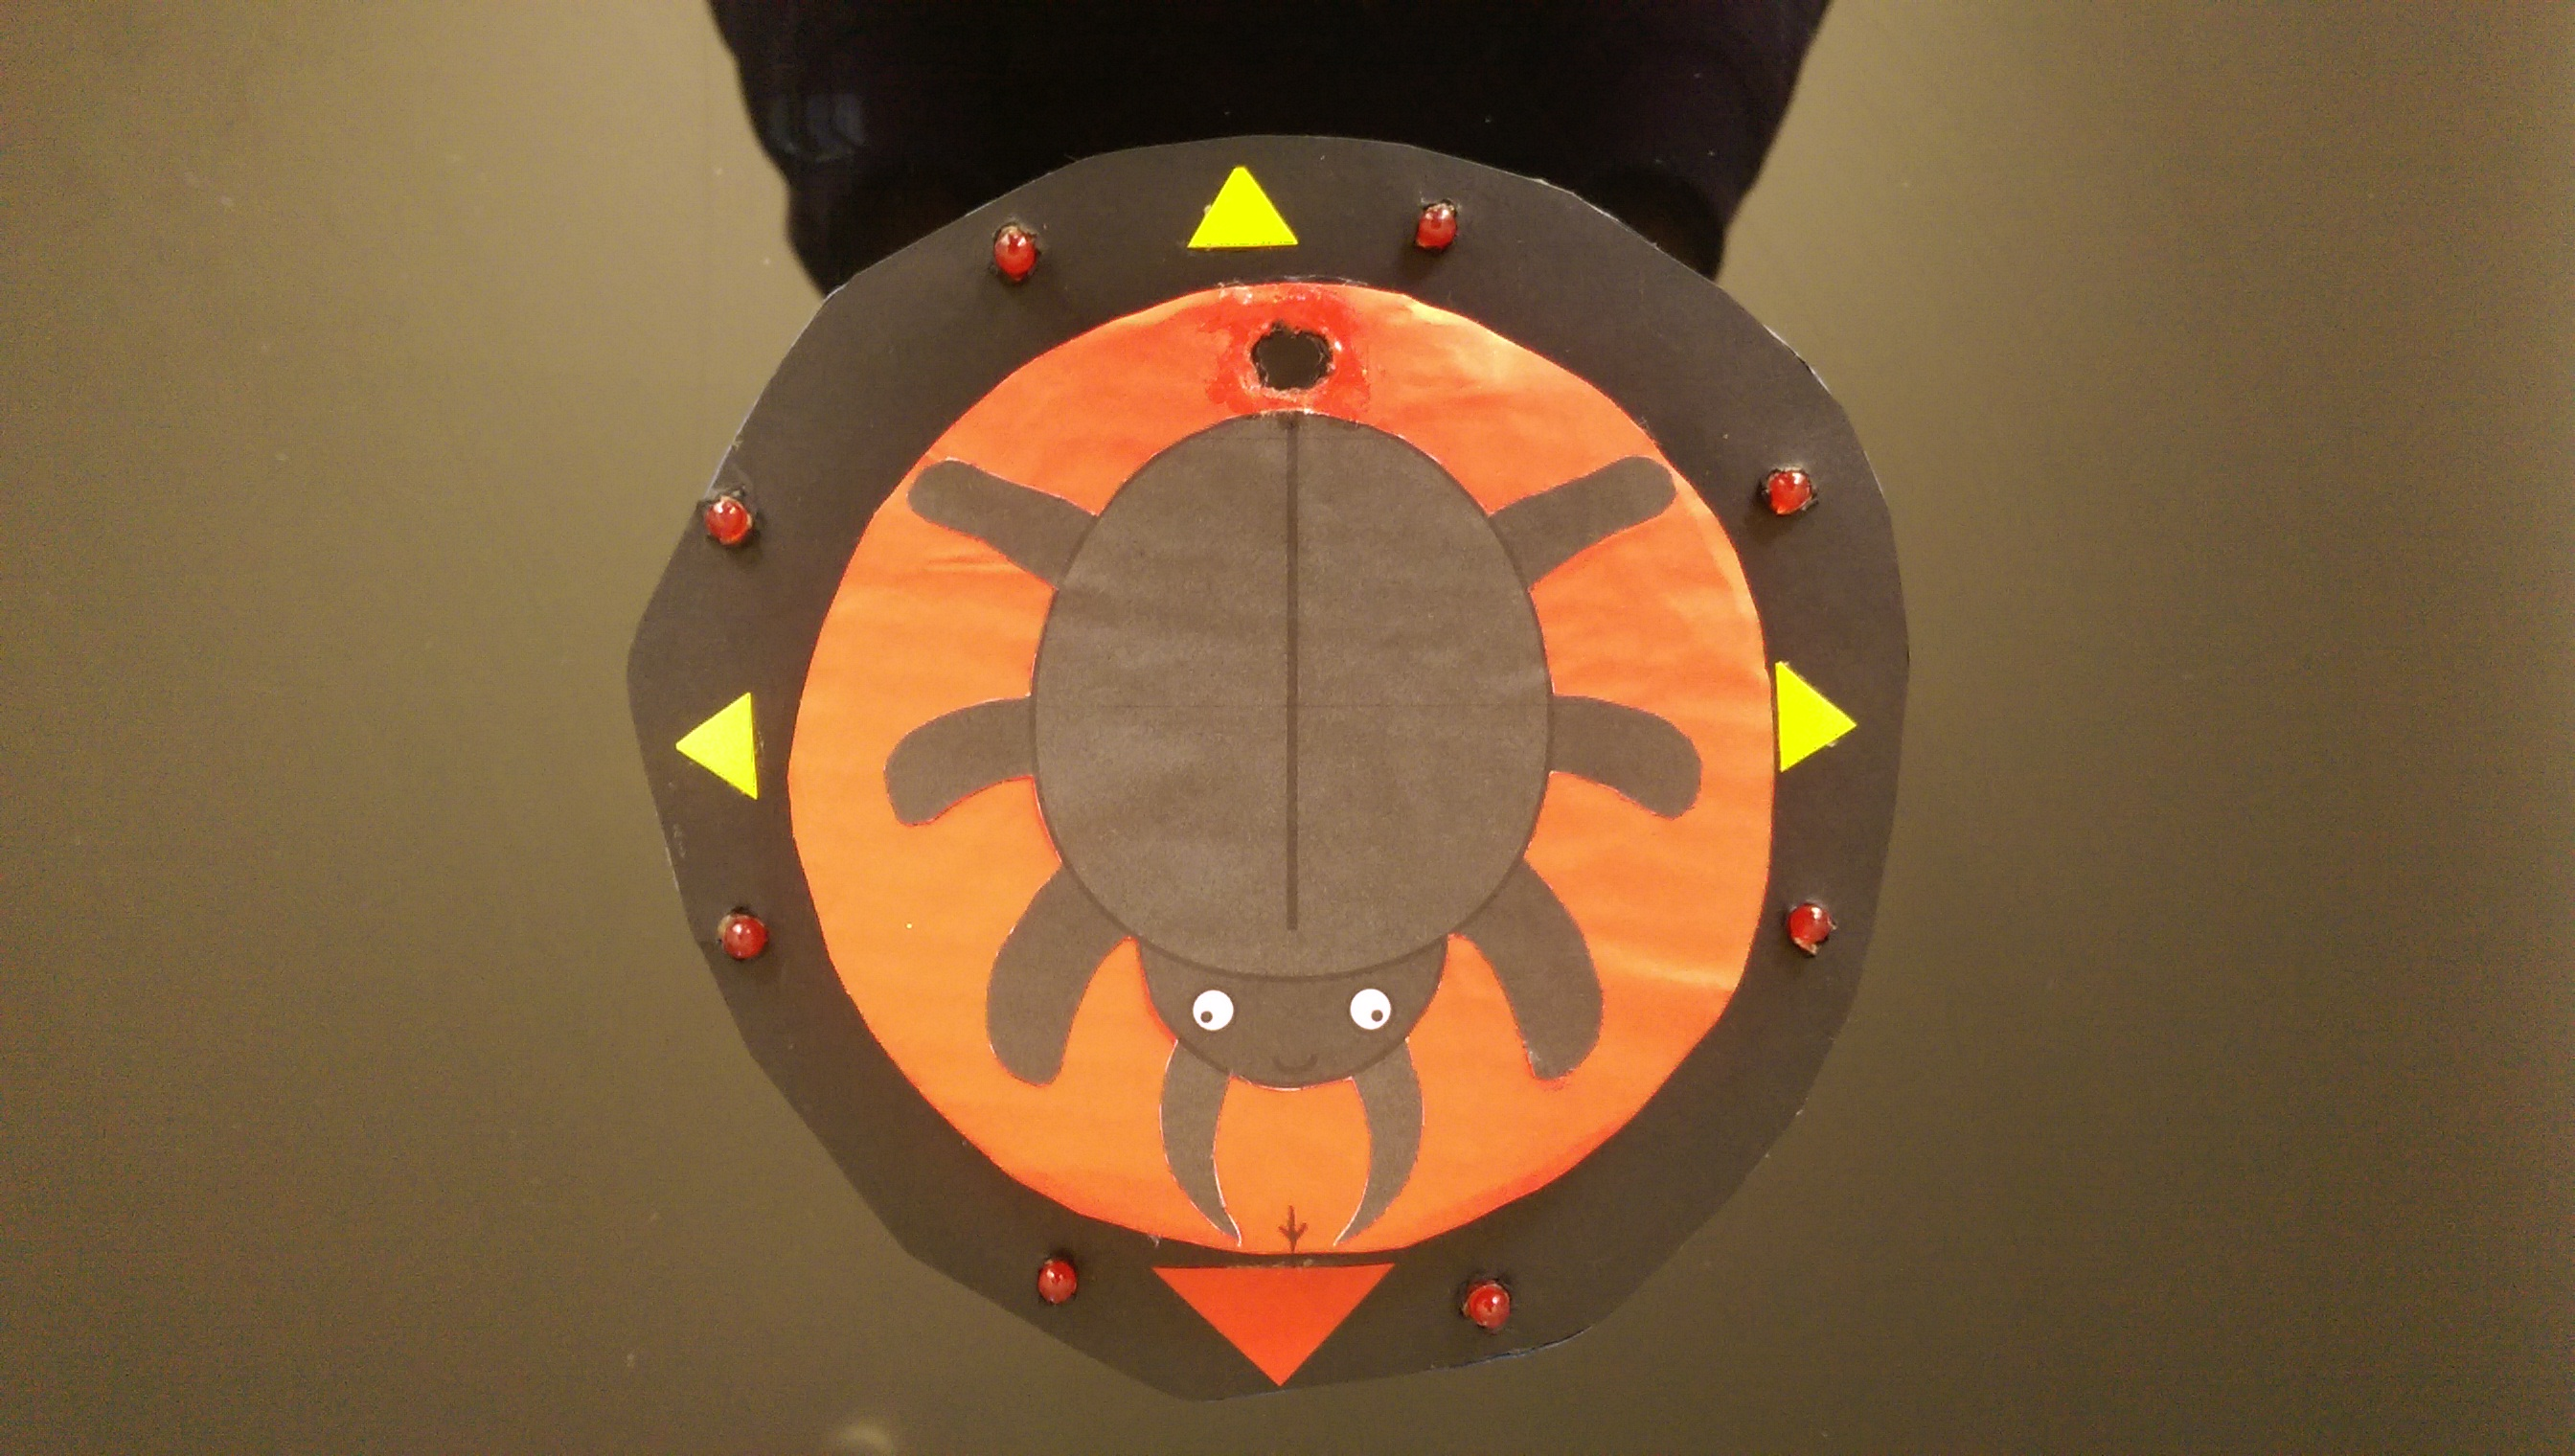
\includegraphics[width=\textwidth]{controller.jpg}
\caption{The Hotrod game controller}
\label{fig:controller}
\end{figure} 
The controller is used by rotating a disc with an image of Hotrod on so that he is facing in the direction of intended travel. An image of the controller is shown in Figure~\ref{fig:controller}.


\section{Evaluation Process}
Due to the circumstances of the review session, the controller was only reviewed by one evaluator. As a result, it is likely that there will be further usability problems that were not reported by the evaluator. The review would have been more effective if there were between three and five evaluators~\cite{nielsen:evaluation}. The review process was otherwise carried out by following the guidelines provided by Nielsen~\cite{nielsen:how}.

\section{Heuristics}
The heuristics used are described in table~\ref{table:heuristics}. They are adapted from Nielsen's heuristics~\cite{nielsen:heuristics} and Pinelle's heuristics~\cite{pinelle:heuristic} in order to be made more appropriate for a usability analysis of a game controller.

\begin{table}
\centering
\begin{tabular}{| l | p{6cm} |}
\hline
\textbf{Heuristic} & \textbf{Application to Game Controller} \\ \hline
Responsiveness of controls & Inputs on the controller should be reflected promptly in the game \\ \hline
Ease of interpretation of system status & The status of the game and the controller should be made clear and easy to interpret without distracting from the game \\ \hline
Recognition over recall & The functions of each component of controller should be easily recognisable, rather than needing to remember what each button does \\ \hline
\end{tabular}
\caption{Heuristics used in usability analysis of the controller}
\label{table:heuristics}
\end{table}

\section{Design Issue 1: Purpose of LEDs Unclear}
The reviewers indicated that the purpose of the LEDs was unclear. The LEDs indicate where the walls are. Their use was likely unclear as they do not enhance the gameplay or provide the player with any useful information. The player often won't have time to look down at the controller. Furthermore, the information that the LEDs are intended to convey is displayed on-screen in a clearer and more helpful manner.

\subsection{Proposed Solutions}
The reviewer reported initially believing that the LEDs were indicating the orientation of the controller. This may indicate that this is a more intuitive and clear use of the LEDs. Furthermore, providing an indication of the direction the controller is registering will be more useful to the player, as it can sometimes be unclear which direction is active due to the nature of the controller's free rotation. 

An even more effective use of the LEDs could be to flash when the player is powered up. This could be registered in the player's peripheral vision without requiring them to look away from the screen and process complex information.

\section{Design Issue 2: Controls Feel Unresponsive}
The controller was reported to feel unresponsive: you must rotate the controller \textit{before} the desired turning, otherwise the character will continue past. The observations are described in Table~\ref{table:issue2}. This could be caused by a disconnect between the game's design and the controller's design. The game compensates for the character's continuous movement by allowing input to be registered before a turning, allowing the player to feel in control. Not only is this the optimal way to play, but the time taken to physically manipulate the controller means that this play-style is enforced. However, this results in an inconsistency between the controller's image and the game's image.

\begin{table}
\centering
\begin{tabular}{| p{6cm} | p{6cm} |}
\hline
\textbf{Heuristic} & \textbf{Observation} \\ \hline
Responsiveness of controls
 & The controller creates a feeling of unresponsiveness. It feels natural to turn the controller at the time the character is intended to turn. However, doing this results in the movement not being registered until after the turning. \\ \hline
Ease of interpretation of system status
 & The way the controller should be used is confusing. If the optimal play-style is used, the controller does not match what is seen on screen. This makes the player feel that turning the controller at the instant a direction change is desired is how it should be used, resulting in issues concerning lack of responsiveness. \\ \hline
\end{tabular}
\caption{Observations relating to heuristics relevant to this design issue}
\label{table:issue2}
\end{table}

\subsection{Proposed Solutions}
It may not be appropriate to adjust the game so that it responds to input differently, primarily because this would reduce the responsiveness and control provided when playing the game using different control methods. Therefore, reducing the controller's size so that the distance it needs to travel to rotate is smaller may help increase the feeling of responsiveness. The image of Hotrod still won't correspond to the image on screen most of the time, but it can be thought of as instructing him where to go next.

\section{Conclusion}
The usability of the controller may be increased by applying the proposed changes to the design in order to address the issues raised during the evaluation.

\bibliographystyle{ieeetran}
\bibliography{comp140-evaluation}

\end{document}
